\section{Motivating Examples}
\label{sec:motivation}

As mentioned in Section 1, the programmer writes a Pig Latin program in an imperative style with high level declarative data transformation operations and mapping each operation to am identifier which can be later re-utilized and reordered. The program is compiled to parallel map-reduce jobs through generation of logical and physical plan. The underlying compilation is hidden from the user and abstracted away with the simple semantics of Pig Latin. The correctness of the compilation is of prime importance to state that underlying map-reduce jobs produce the intended final output of the program.
We now present some examples to motivate our approach.

\subsection{Example 1:}
\label{subsec:example1}

The following example\cite{gates2009building} describes a simple Pig Latin program that takes two data sources file1 and file2 as input. performs a series of data transformations on them and finally stores the output.
\begin{lstlisting}
	A = LOAD 'file1' AS (x,y,z);
	B = LOAD 'file2' AS (t,u,v);
	C = FILTER A BY y>0; 
	D = JOIN C BY x, B by u;
	E = GROUP D BY z;
	F = FOREACH E GENERATE group, COUNT(D);
	STORE F into 'output';
\end{lstlisting}

In the above example two files are loaded into variable A and B. A is filtered by a predicate and the data transformation operation is assigned to C. D represents the JOIN operation of C and B. The GROUP BY operation is assigned to the identifier E and finally a count aggregate function is applied to the relation E and the output is stored into F and stored.

\begin{figure}
\begin{center}
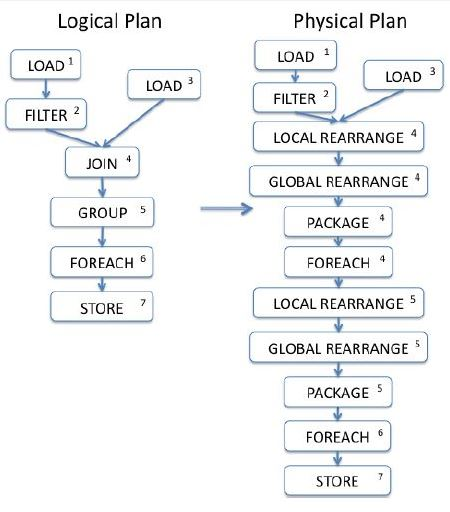
\includegraphics[scale=0.5]{Images/LogicalPhysicalPlan.JPG} 
\end{center}
\caption{\textbf{Logical - Physical Plan\cite{gates2009building}}}
\end{figure}
In Figure 1 it shows how the program from the example gets compiled to the logical plan and physical plan. Each data transformation operation gets mapped one to one to each node in logical plan. Each logical operator is annotated with a number id corresponding to the operation defined in the program. The logical plan is then translated into a physical plan where the GROUP BY operation is divided into a series of physical operators - LOCAL REARRANGE, GLOBAL REARRANGE, PACKAGE operations and JOIN operation comprises of the same physical operators followed by a FOREACH operation. Corresponding logical and physical operators are annotated with the same id.
